\section{国内外研究现状分析}

\subsection{研究方向概述}
简要介绍论文研究方向主要研究分支,每个分支做了哪方面的研究

\begin{figure}[h]
  \centering
  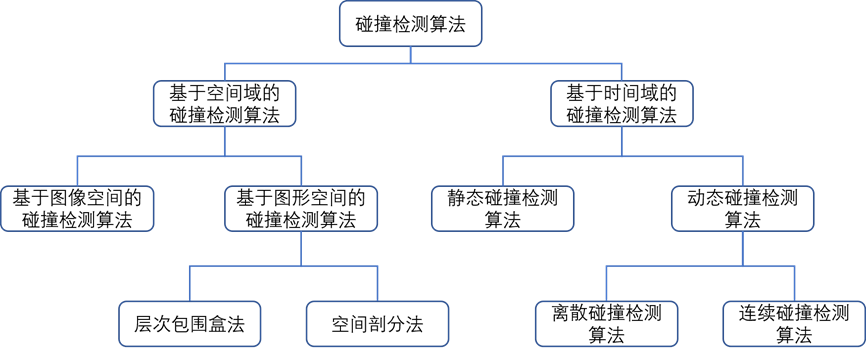
\includegraphics[width=\linewidth]{fig_direction}
  \caption{碰撞检测算法分类}
\end{figure}

\zhlipsum[1]

详细介绍各分支的理论、方法或技术研究现状

\subsection{XXX研究现状}
XXX研究现状

\subsubsection{方向1研究现状}
\subsubsection{方向2研究现状}
\subsubsection{方向3研究现状}

\subsection{XXX研究现状}
XXX研究现状

\subsection{XXX研究现状}
XXX研究现状

\subsection{研究现状总结与分析}
针对本论文遇到的问题,XXX等人的方法存在XXXX问题。
\textbf{\color{red}
(用2页左右的篇幅,对文献综述所罗列的研究现状进行总结和分析,并列举与论文密切相关的几项工作)}

\subsubsection{论文研究领域存在的问题}
论文研究领域存在哪些尚未解决的问题
\subsubsection{论文研究领域的发展趋势}
论文研究方向的未来发展趋势
\subsubsection{研究现状分析结论}
描述哪些问题是本论文需要解决的

\begin{table}[ht]
  \caption{Test table}
  \renewcommand{\arraystretch}{0.8}
  \centering
  \begin{tabular}{l l}
    \midrule
    Title & Column \\
    \midrule
    1 & 2\\
    \midrule
  \end{tabular}
\end{table}

\clearpage
